\chapter{Interactions between the Stratospheric Polar Vortex and Atlantic circulation} 
\begin{quotation}
  Much of the work contained in this chapter is based upon xxx,
  published in \emph{Journal of Climate}, although the analysis
  presented here has been significantly extended.
\end{quotation}

\label{cha:moments}


\section{Introduction}
Chapter 3 demonstrated that the appearance of SSWs varies on multi-decadal timescales in a pi-control simulation. Given the well studied downward influence of vortex variations over the Atlantic sector (see section \ref{sec:Downward_influence}), a natural question that follows from this finding is to what extent do these multidecadal signals influence modes in tropospheric and surface climate? The majority of studies that have examined the associations between the stratospheric polar vortex and surface anomalies have considered their in-season impact, however the Atlantic region exhibits key modes of multi-decadal variation in ocean circulation and SSTs (the AMOC and the AMV, section \ref{sec:multi-decadal_background}) which are in turn key drivers of climate variation. In this chapter, we assess the influence of vortex anomalies on surface and Ocean variations across multiple timescales (in-season to multi-decadal)
in the same pi-control simulation as analysed in chapter 3. We also utilise the relationship between the vortex and AMOC established in this model to estimate the contribution of the stratosphere, namely the 8 year SSW hiatus interval in the 1990s, to recent trends in AMOC observations.

The effect of decadal to multi-decadal scale variation in the vortex on the surface has been considered in previous works, but its true nature is not fully understood. \cite{manziniStratospheretroposphere2012} examines decadal fluctuations in SSW events in a 260 year prescribed SST simulation of a GCM and analyse impacts of these signals at the surface. They show that decadal vortex variability excites similar timescale variations in surface temperature and sea ice coverage between Greenland and Norway over the Atlantic sector. They propose this connection to be indicative of a delayed response of the AMOC to stratospheric forcing via the NAO which  subsequently influences northward Atlantic heat transfer and sea ice melt rates as well as surface temperatures anomalies. \cite{haaseImportance2018} analyse the in-season impact of SSW events on the strength of deep convection in the North Atlantic that occurs through the impact of SSWs on the NAO using a model (CESM1 WACCM). The study notes the presence of an anomalously shallow  mixed layer depth in the Labrador Sea following an SSW event. 

An association between stratospheric polar vortex variability and the AMOC on decadal timescales has also been previously investigated \citep{reichlerStratospheric2012, Schimanke2011} but the mechanism of its influence remains unclear. For example, \cite{reichlerStratospheric2012} examine the response of the AMOC to strong and weak polar vortex events and show a lagged response in the AMOC leading to oscillatory responses. They propose a pathway involving alterations of wind stress and ocean-atmosphere heat flux anomalies in the West Atlantic due to the changed NAO patterns following the vortex events. The effect is seen in both reanalysis and to some extent in a suite of CMIP5 models. An impact of long-term changes in the NAO on the strength of the AMOC is supported by a number of studies \citep{visbeckOcean1998, delworthImplications2000, delworthMultidecadal2000, edenMechanism2001}. Most recently \cite{delworthImpact2016} used a set of idealised GCM experiments in which they impose a perpetual ocean-atmosphere heat flux pattern associated with different NAO phases. They find significantly different AMOC mean states depending on the imposed pattern (a stronger AMOC under positive NAO flux conditions than a control simulation). 


\section{Data And Methods}
\subsection{Model Configuration and Observation Data}

We analyse output from the same GCM simulation as presented in chapter 3 - the pi-control simulation of UKESM (see section \ref{sec:model_config}). As in chapter 3, we choose the pi-control due to the length of integration relative to the timescales we wish to consider and to analyse the internal variability of the system in this model. 

To estimate the contribution of stratospheric variations to recent observed AMOC trends we also make use of observation based datasets of the atmosphere and oceans. First, we utilise the reanalysis data from the European Centre for Medium-Range Weather Forecasts (ECMWF): ERA5 \citep{hersbachERA52020} for observation based geopotential height (GPH) fields. Similar to its predecessor, ERA-Interim (section \ref{sec:ERA_data}), ERA5 consists of a set of observations assimilated through 4D-var using ECMWF Integrated Forecast System (IFS). However, ERA5 utilises the latest version of the IFS which operates at a greater horizontal grid resolution to ERA-Interim (31km vs 80km) as well as a higher vertical resolution and maximum height (60 levels up to 10hPa vs 137 levels to 1 hPa) \citep{hersbachERA52020}. Most relevant for stratospheric representation is the inclusion of an improved gravity wave parameterisation scheme in the latest IFS \citep{orr} and \cite{hersbachERA52020} reports a marginal improvement in the predictability of SSW events in the latest IFS compared to its predecessors. Despite these 

We choose to utilise ERA5 as opposed to ERA-Interim for analysis in this chapter as we consider observations of the AMOC and the vortex up to near present day. ERA5 provides data up till present day while ERA-Interim has been discontinued as of 2019 so ERA5 is a preferable dataset in this case. 

Second, the Rapid Array Dataset which provides time-depth profiles for the meridional overturning mass streamfunction in the Atlantic region at 26$^{\circ}$N \citep{moatAtlantic2020}. These data are measured through a combination of ocean mooring, ship based, satellite and submarine telephone cable observations to estimate the strength of primary contributions to the meridional overturning circulation: Ekman transport (through wind stress), transport through the Florida Straits and transport driven by EW density gradients between the American and African continents \citep{mccarthyMeasuring2015}.

\subsection{Model Diagnostics}
\label{sec:model_diagnostics_surface}
We utilise the Northern Annular Mode (NAM) as a metric for the strength of the vortex as used by \cite{baldwinStratospheric2001a} as well as numerous subsequent studies. The NAM is defined as the 1st principle component of the zonal mean, deseasonalised geopotential height field evaluated at latitudes north of $20^{\circ}N$ over the NH winter season (Nov-Mar) on a given pressure level. To measure the vortex strength we evaluate the NAM on a level in close proximity to the vortex edge, 10hPa, and the resulting index is henceforth known as NAM$_{10}$. We choose to utilise a continuous vortex metric for this work as opposed to the event based measured used in chapter 3 as the NAM captures both types of anomalous vortex behaviour (strong and weak). Cross spectral analysis of the SSW time-series and the QBO (figure \ref{fig:SSW_low_rate_QBO}) suggested an important role of SSW hiatuses in multi-decadal modes of variation. As a result, a continuous metric that distinguishes between a weak, strong and neutral vortex is highly useful for this analysis. An individual vortex event (either strong or weak) is recorded when the daily NAM$_{10}$ crosses +1.5 (strong) or -2 (weak). The day on which this reversal occurs is referred to as the central date. After this date, the NAM$_10$ must recover to neutral (between -2 and 1.5) for a period of at least 10 consecutive days (which is the approximate radiative timescale of the mid-stratosphere) before another event can be recorded. The strong threshold value for events is chosen in accordance with the methodology of \cite{baldwinStratospheric2001a} and the weak threshold selected such that it results in approximately the same rate of weak events (SSWs) as is reported in chapter 3 (figure \ref{fig:SSW_histogram}) using the same simulation of UKESM but with a zonal wind definition of SSWs (0.54 events/winter).

We also use the NAM$_{10}$ to derive an index for the appearance of intervals of consecutive winters which show persistent vortex behaviour. The persistent NAM$_{10}$ interval index is defined as the annual mean Nov-Mar NAM$_{10}$ (which gives a measure of vortex strength for each winter) which has additionally been smoothed using a Gaussian filter. This smoothing is carried out through a convolution of the time-series with a 1D Gaussian kernel in the time domain given by

\begin{equation} \label{Gaussian_filter}
f(t, \sigma) = \frac{1}{\sqrt{2 \pi \sigma^2}} e^{-\frac{1}{2}\big(\frac{t}{\sigma}\big)^2}
\end{equation}

Where $\sigma$ is the standard deviation of the distribution defined by the kernel. We choose $\sigma$ = 2 years following the method of \cite{reichlerStratospheric2012} and as a method analogous to the 5 year smoothing applied to an SSW timeseries in chapter 3. The selection of $\sigma = 2$ years allows contributions to the smoothed value from values approximately 7 years either side of the central year as the value of the Gaussian window decays to near 0 approximately $3.5\sigma$ from its mean. However the largest contributions come from 3-4 years either side of the central year. This allows the smoothing to capture instances of $\sim 6-8$ consecutive years with persistent vortex behaviour, a similar length to intervals observed in reanalysis (e.g. the 1990s, \cite{pawsonCold1999}). We subsequently define persistent NAM$_{10}$ intervals, when the vortex exhibits the same type of behaviour for a number of consecutive years, using extreme values of the smoothed NAM$_{10}$ index. A persistent NAM$_{10}$ interval is recorded when the smoothed NAM$_{10}$ index value falls within the top 5 percentile values. Once such an interval occurs, another cannot be recorded for 15 years after to avoid choosing multiple central years within the same interval. Using 5 percentile values gives approximately the same rate of persistent vortex intervals as is reported in \cite{reichlerStratospheric2012} so we proceed with this threshold throughout for a direct comparison with this study. Tests were also carried out to assess the sensitivity of our results to this threshold and are reported in section 3.

We define an AMOC index following the procedure in \cite{reichlerStratospheric2012}. The AMOC is defined using overturning streamfunction field averaged in the Atlantic sector. At each time point the AMOC index is the maximum streamfunction value at any depth at a chosen latitude. We evaluate the index at 30N, 45N and 50N and measure the response and co-variability with the SSW timeseries and other climate indices defined below. We derive the observed AMOC index from the Rapid Array data as the maximum MOC at each time point at 26N. We also utilise a definition of the North Atlantic Oscillation from \cite{hurrellNorth2003}. The NAO index is defined as the 1st principle component (PC) of the Dec-Mar MSLP in the region $20^{\circ}-80^{\circ}N, 90^{\circ}W-40^{\circ}E$. The pc is calculated by taking the first empirical orthogonal function (EOF) of deseasonalised MSLP anomalies and projecting this EOF onto the anomaly field. We additionally derive an Ocean-Atmosphere heat flux field defined as the sum of latent and sensible heat fluxes between the ocean surface and the atmosphere (i.e. positive values indicate exchange of heat from the ocean to the atmosphere). We derive an index for the occurrence of deep convection anomalies in the equatorial eastern Pacific region. This index is defined by the top of atmosphere outgoing longwave radiation (OLR) averaged over the box 10$^{\circ}$\,S–10$^{\circ}$\,N, 240$^{\circ}$\,–290$^{\circ}$\,E. The OLR field is utilised as it acts as a proxy for the occurrence of convection anomalies - When deep convection is enhanced, cloud top height is increased and therefore OLR is reduced. The East Pacific box is selected following a sensitivity analysis to establish the region which exhibits 90 year timescales variations in OLR. It is also a similar region to studies which consider east pacific ENSO patterns which is identified as a separate mode of variability to the traditionally used central pacific ENSO region \citep{johnsonHow2013}.

Finally, we utilise the same QBO metric as in the wavelet analysis of chapter 3 (see section \ref{sec:model_diagnostics}. This is defined as the Zonal Mean Zonal Wind (ZMZW) averaged over the latitude range 5$^{\circ}$\,S–5$^{\circ}$\,N,  and the pressure level range 15-30hPa. As with chapter 3 we also consider the Hilbert amplitude of the deep QBO as an instantaneous amplitude metric (see equations \ref{eq:hilbert1}-\ref{eq:hilbert3}). 

\section{In-season surface responses to anomalous vortex events}
We begin by diagnosing the in-season response to anomalous vortex events exhibited by surface variability in the model to assess its suitability for studying interactions on longer timescales. Figure \ref{surface_comp_all} shows the mean sea level pressure (MSLP) composite differences between strong and weak polar vortex years (figure \ref{surface_comp_all}, top row). The composites have been determined by selecting MSLP values associated with events in which the daily NAM$_{10}$ values cross +1.5 (strong) or -2 (weak) (see section \ref{sec:model_diagnostics_surface}). The composite differences demonstrate a significant lagged MSLP response, with strong (weak) vortex years  corresponding to a positive (negative) NAO pattern, in agreement with previous model and observational studies (see section \ref{sec:Downward_influence}). The NAO anomalies peak in magnitude at a lag of 1-2 months following the vortex anomalies with significant anomalies still visible for up to 3 months. There is also a weak positive NAO pattern that leads the vortex anomalies by up to one month ($-1 - 0$ month lags). This may be an indication that an anomalous NAO pattern is a precursor for an anomalous vortex, or it could be a response to the initiation of the vortex anomaly since this usually commences in the upper stratosphere and pre-dates the event's central date defined at 10 hPa. Further exploration of this weak NAO signal is outside the scope of the analysis presented here. Additionally, a much stronger significant positive anomaly over the Aleutian low (AL) region is evident in the month leading up to the vortex anomaly. This signal has been widely studied \citep{raoModulation2019a} and links the intensity of the AL to the strength of vertically propagating planetary waves that subsequently interact with the stratospheric vortex and influence its strength (section \ref{sec:external_influence_AL}). Analysis in chapter 3 examined this coupling using the same pi-control simulation as presented here and found a similar statistically significant relationship between the AL and the frequency of SSWs but the regression coefficients were small in comparison with the QBO influence. Here the association between the AL and the vortex strength appears marginally stronger (r = 0.39 with the NAM$_{10}$) which may be due to the NAM's ability to capture both types of vortex anomalies (strong and weak). In chapter 3 we also showed that the AL exhibited minimal decadal to multi-decadal variability that was coherent with the decadal to multi-decadal variability of the vortex (\ref{fig:AL_wavelet} and for this reason the role of the AL is not considered in detail in this chapter.

\begin{center}
\begin{figure}[h!]
\noindent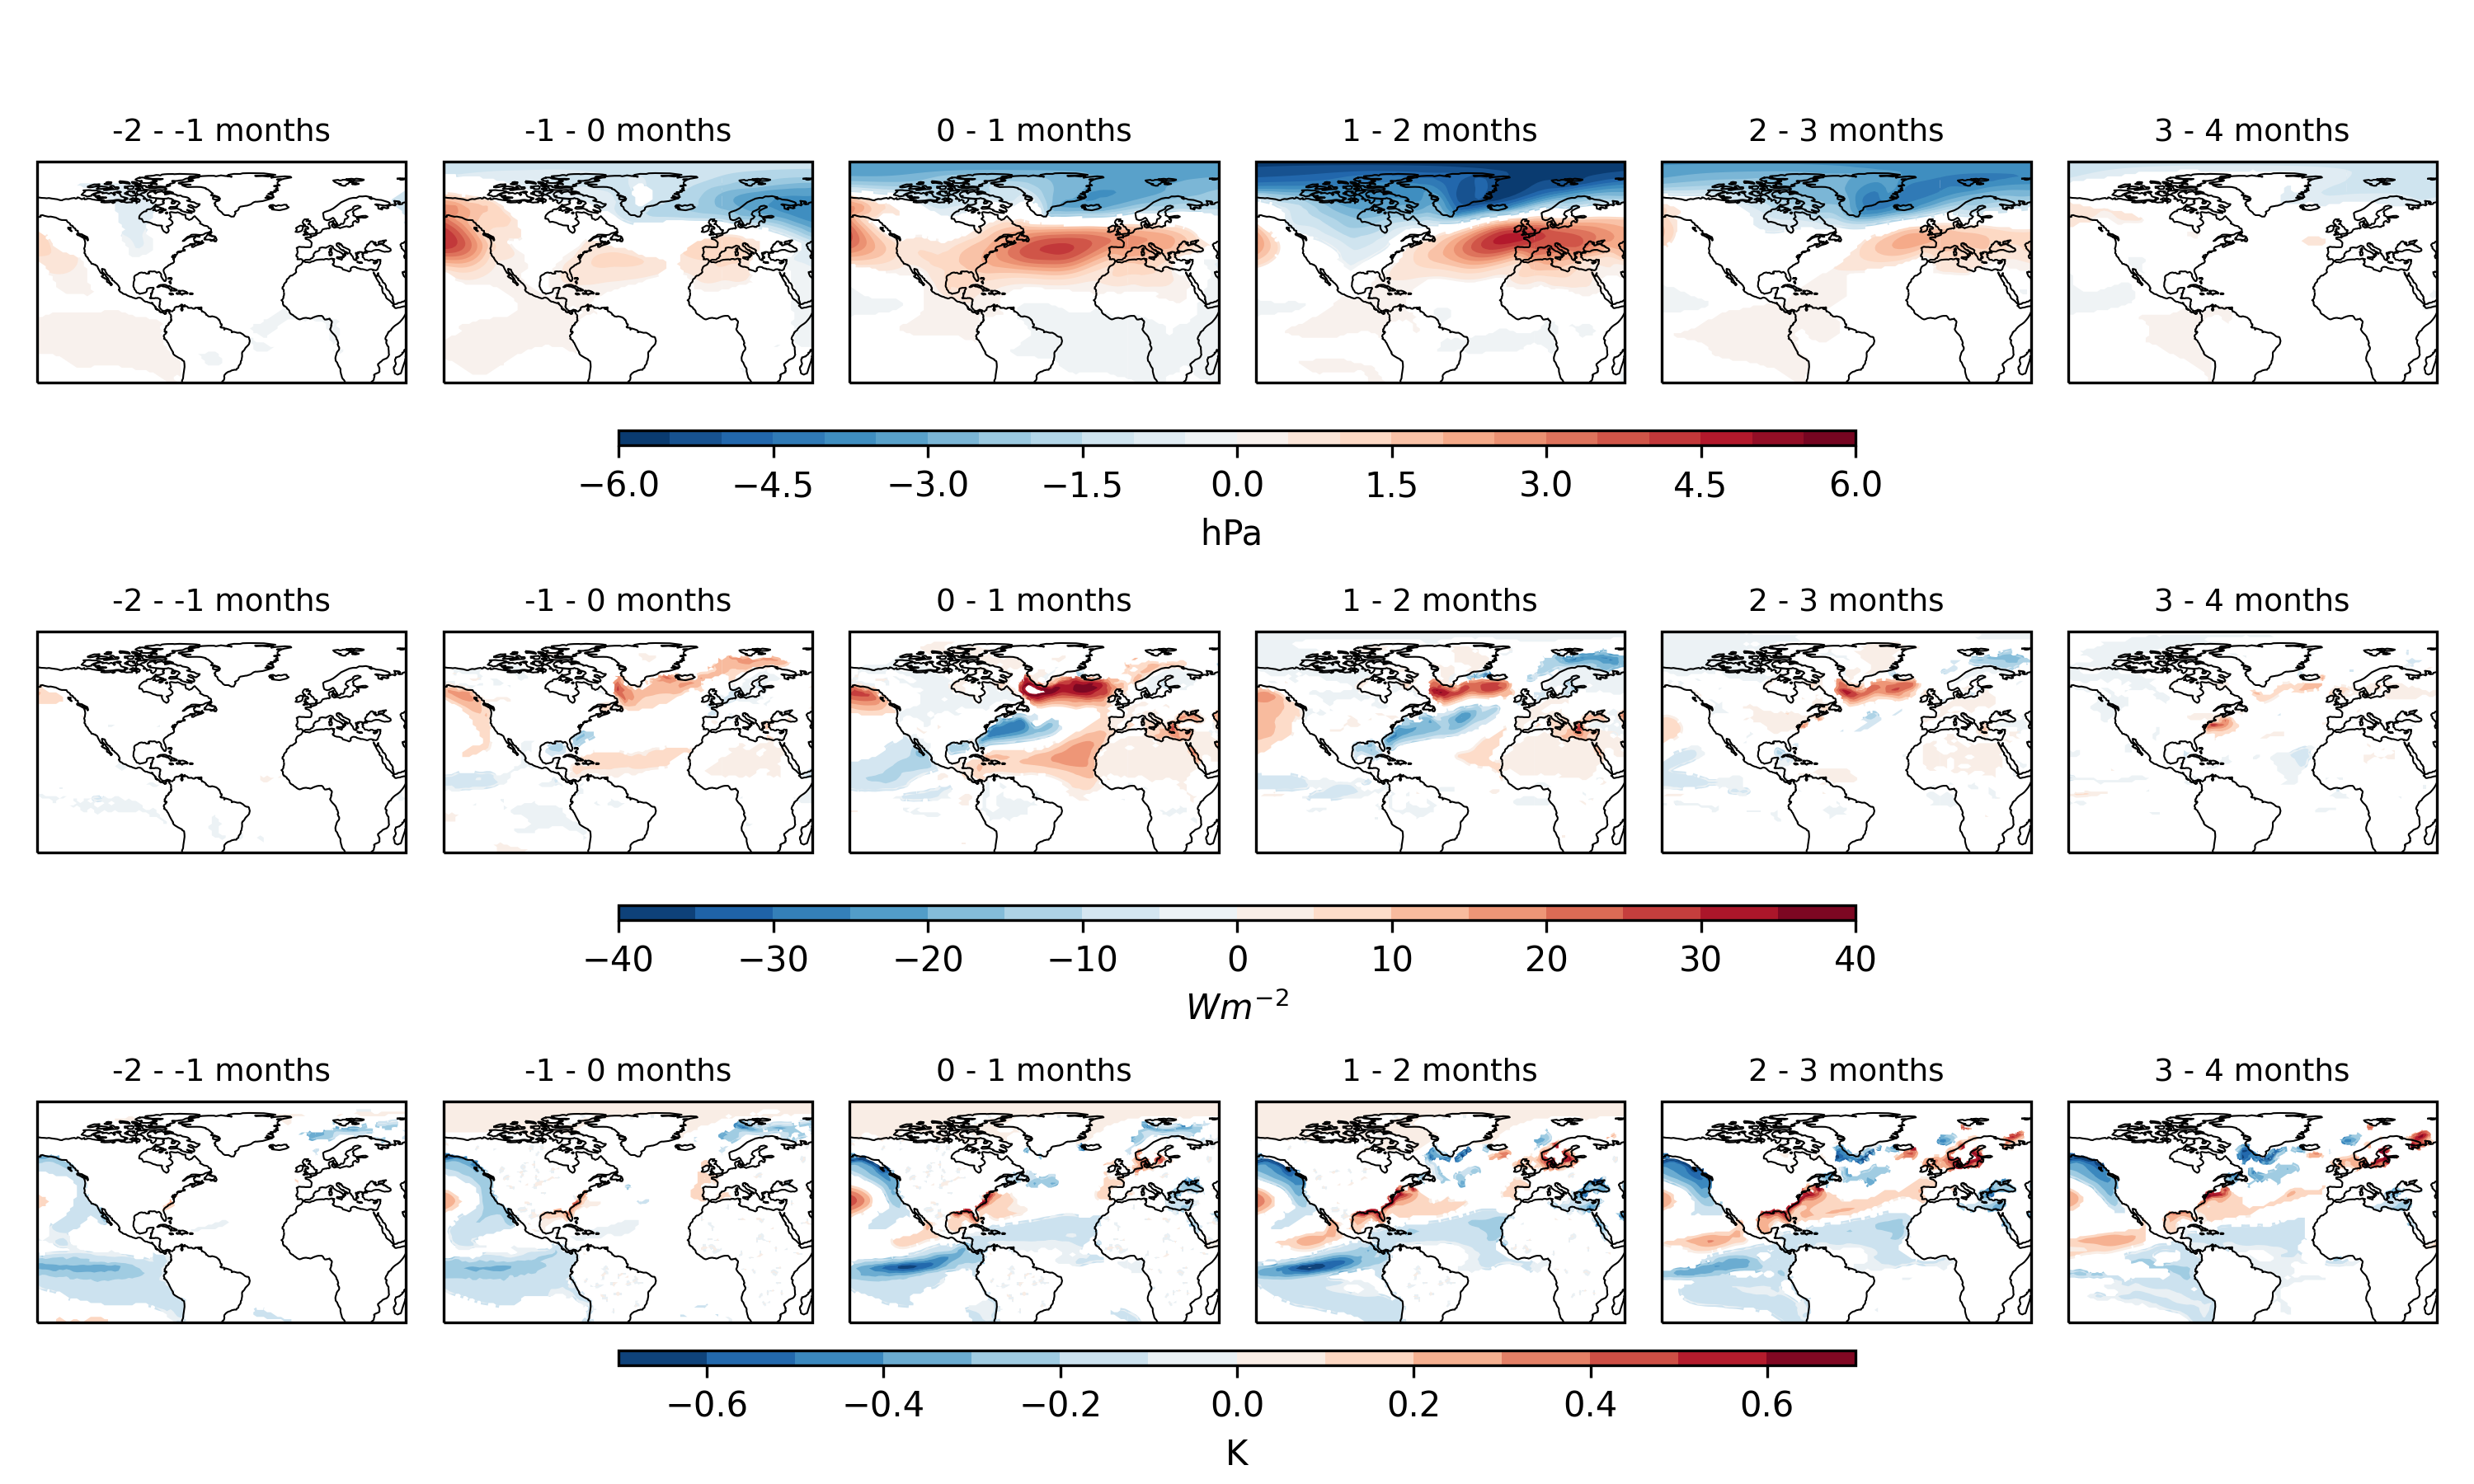
\includegraphics[width = \linewidth]{Figures/Figures-surface/in_season_response_NAM_combined.png}
\caption{Surface patterns associated with anomalous winter stratospheric NAM$_{10}$ events. \textbf{Top row}: Monthly mean sea level pressure anomaly, \textbf{middle row}: Ocean-Atmosphere heat flux defined as the sum of latent and sensible heat fluxes and \textbf{bottom row}: SSTs. Coloured shading shows where the composite differences between strong and weak NAM$_{10}$ events are statistically significant at the 95\% level under a 2 tailed students t-test. The title of each sub-figure indicates the month range relative to the central date of each NAM$_{10}$ anomaly. Signals at negative times indicate that the surface anomaly leads the stratospheric NAM$_{10}$ anomaly. Signals at positive  times indicate that the stratospheric NAM$_{10}$ anomaly leads the surface response.}
\label{surface_comp_all}
\end{figure}
\end{center}

The model also exhibits significant responses in ocean-atmosphere heat flux (figure \ref{surface_comp_all}, middle row). The largest flux anomalies are seen within 30 days (lag 0-1 month) and their spatial pattern resembles that of a North Atlantic tripole with positive anomalies over the Labrador sea and between Greenland and Western Europe, negative anomalies off the east coast of the USA and a second positive anomaly off the coast of north east Africa. This pattern is consistent with the model response found by \cite{reichlerStratospheric2012} to anomalous stratospheric NAM$_{10}$ events as well as the pattern associated with positive NAO phases in \cite{delworthImpact2016}. As with the MSLP composites, there are visible anomalies 30 days leading up to the identified events (lag -1 - 0 months) both over the North Atlantic and Pacific regions. The Atlantic pattern may correspond to early responses to a disrupted or strengthened vortex. The Pacific anomalies preceding events are considerably smaller than the Atlantic anomalies and are concentrated over the Aleutian low region.

The SST response to anomalous stratospheric NAM$_{10}$ events (figure \ref{surface_comp_all}, bottom row) over the North Atlantic lags behind the heat flux anomalies by around 2 months, with the largest amplitude anomalies at around 2-4 month lags.  The anomaly pattern resembles that of the heat flux anomalies (with a change of sign), consistent with a mechanism in which the SSTs respond to the anomalous heat fluxes. A prominent negative tropical East Pacific anomaly is obvious in the months leading up to anomalous vortex events together with  anomalies that resemble the Pacific Decadal Oscillation (PDO) in the region of the Aleutian Low \cite{mantuaPacific1997} and these features persists for several months. Variability in this region is dominated by ENSO variations and a significant body of work has proposed teleconnections between ENSO and vortex strength, consistent with the type of association exhibited here (see section \ref{sec:external_influence_SSTs}), i.e. negative (positive) SSTs or la Ni\~{n}a (el Ni\~{n}o) conditions associated with an anomalously strong (weak) vortex. 




%%% Local Variables:
%%% mode: latex
%%% TeX-master: "thesis"
%%% End:







